%! Author = sudharsangopalakrishnan
%! Date = 8/4/21

% Preamble
\documentclass[11pt]{article}

% Packages
\usepackage{amsmath}
\usepackage{graphicx}
\usepackage{xcolor}
\graphicspath{ {../../ChanR EDA/} }


\title{ChanR GMO Project: Exploratory Data Analysis}
\author{Sudharsan Gopalakrishnan}

% Document
\newcommand\mymaketitle{%
    \begin{titlepage}
        \begin{center}
            \vspace*{\fill}
            {\LARGE \textbf{\textcolor{blue}{ChanR GMO Project: Exploratory Data Analysis}} \par}
            \vskip 1em {\Large Sudharsan Gopalakrishnan \par}

            \vspace*{\fill}
        \end{center}
        \small \centering This document was created using the \LaTeX{} programming language.
    \end{titlepage}
}

\begin{document}

    \mymaketitle
    
    \newpage
    
    \section{Overview:}

    \vspace{5}
    The first part of my GMO project is to survey several people
    and ask them questions related to GMOs to get an overall idea
    of their general knowledge of the topic.
    I asked them 18 questions, 17 of which were multiple choice.
    The remaining one asks to write the full form of the word
    GMO\@.
    After surveying them, I performed some data analysis on the data
    I received.
    All the survey data was stored in a Google spreadsheet.
    As I wanted to get more responses overtime, I used a Google
    Spreadsheets API to directly access the data from the spreadsheet
    rather than downloading a csv of the data multiple times.
    Using a Python based Jupyter Notebook, I created a Pandas
    DataFrame and plotted the percentages of the people that got
    each question right and those who got them wrong.

    \section{Survey Questions:}
    \textbf{Notes:}
    Question 2 asks to write the full form of GMOs.
    Because people would have either used or not used
    capitalization in their response the same as each other,
    making a pie unreasonable.
    \subsection{Yes/No Format(1-8):}
    Question 1: Have you ever heard about the word GMOs?
    \begin{center}
        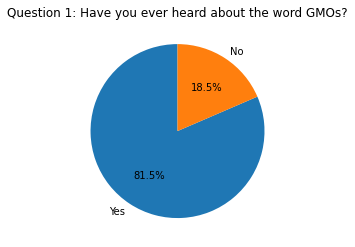
\includegraphics[width=200]{ChanR EDA/q1}
    \end{center}

    \newpage
    Question 3: Are you aware of the objective of GMOs in the market?
    \begin{center}
        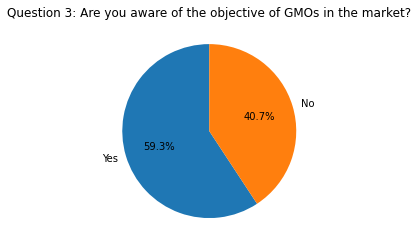
\includegraphics[width=250]{ChanR EDA/q3}
    \end{center}

    Question 4: Are you aware of any health benefits/risks of GMOs?
    \begin{center}
        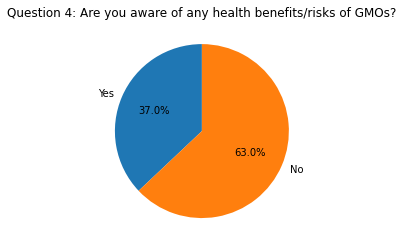
\includegraphics[width=220]{ChanR EDA/q4}
    \end{center}

    Question 5: Are you aware of any products of GMOs today in the market?
    \begin{center}
        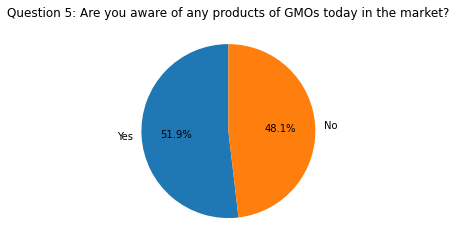
\includegraphics[width=270]{ChanR EDA/q5}
    \end{center}

    \newpage
    Question 6: Are you aware of the similarities AND differences between organic crops and GMOs?
    \begin{center}
        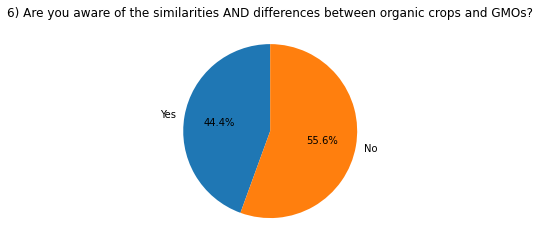
\includegraphics[width=300]{ChanR EDA/q6}
    \end{center}

    Question 7: Are GMOs made by just injecting something with a syringe?
    \begin{center}
        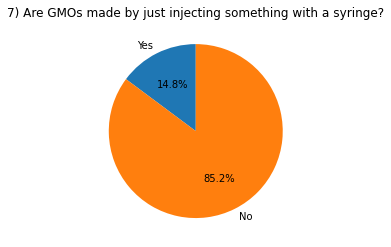
\includegraphics[width=200]{ChanR EDA/q7}
    \end{center}

    \item{Question 8: Are Non-GMO labels used properly on commercial foods today?}
    \begin{center}
        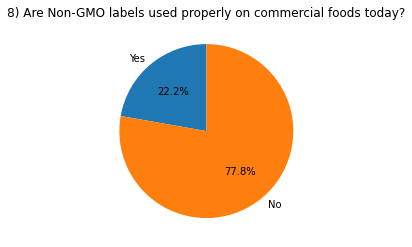
\includegraphics[width=200]{ChanR EDA/q8}
    \end{center}

    \newpage
    \subsection{True/False Format(9-16):}
    \item{Question 9: Organic food is proved to be safer than GMOs.}
    \begin{center}
        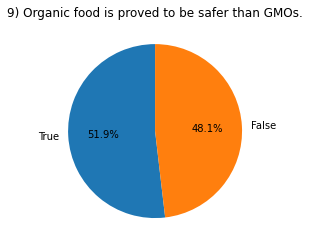
\includegraphics[width=170]{ChanR EDA/q9}
    \end{center}

    \item{Question 10: GMOs are purely artificial.}
    \begin{center}
        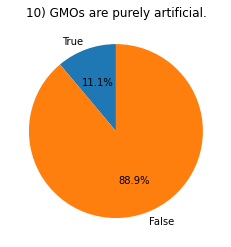
\includegraphics[width=150]{ChanR EDA/q10}
    \end{center}

    \newpage
    \item{Question 11: GMOs are a novel aspect of today.}
    \begin{center}
        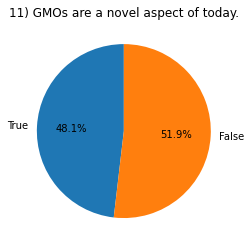
\includegraphics[width=150]{ChanR EDA/q11}
    \end{center}

    \item{Question 12: GMOs are very common in the world today.}
    \begin{center}
        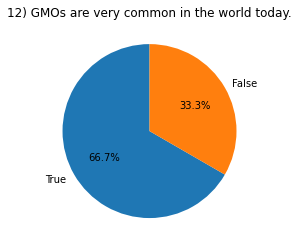
\includegraphics[width=170]{ChanR EDA/q12}
    \end{center}

    \item{Question 13: GMOs can be pest resistant and can therefore reduce the necessity of chemicals.}
    \begin{center}
        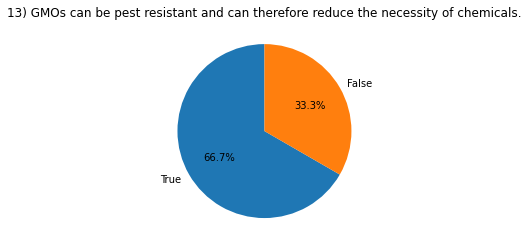
\includegraphics[width=270]{ChanR EDA/q13}
    \end{center}

    \newpage
    \item{Question 14: GMOs are more harmful than beneficial.}
    \begin{center}
        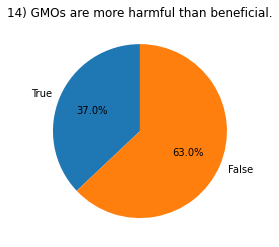
\includegraphics[width=170]{ChanR EDA/q14}
    \end{center}

    \item{Question 15: GMOs have lowered the level of responsibility of farmers to take care of crops in general.}
    \begin{center}
        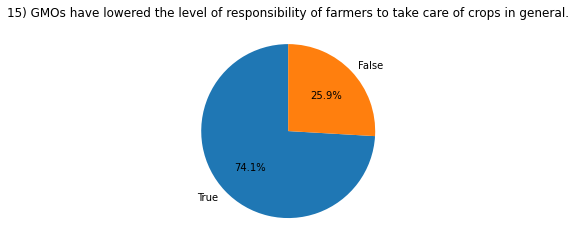
\includegraphics[width=300]{ChanR EDA/q15}
    \end{center}

    \item{Question 16: GMO consumption can cause autism and obesity.}
    \begin{center}
        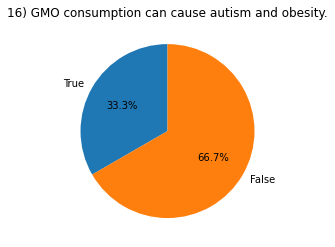
\includegraphics[width=200]{ChanR EDA/q16}
    \end{center}

    \subsection{Yes/No Format(17-18):}
    \item{Question 17: Since the arrival of GMOs have increased the use of GMO-resistant Glyphosate, does this indicate that the use of Glyphosate is better than GMOs?}
    \begin{center}
        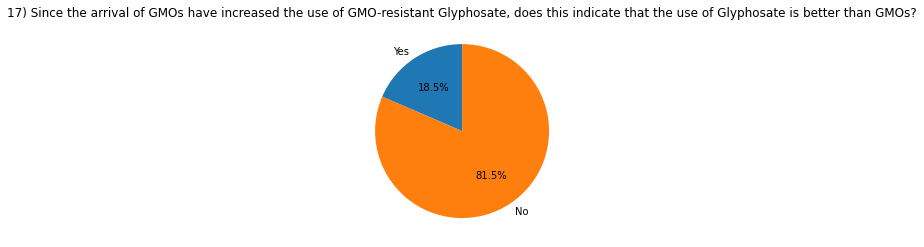
\includegraphics[width=450]{ChanR EDA/q17}
    \end{center}

    \item{Question 18: Are GMOs a solution to issues regarding food sustainability?}
    \begin{center}
        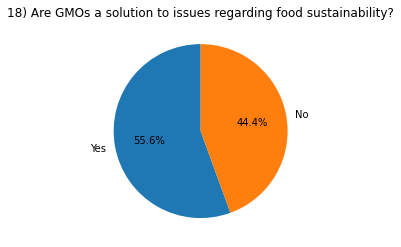
\includegraphics[width=200]{ChanR EDA/q18}
    \end{center}








\end{document}